This layer is associated with reading the MIDI signals and converting it into audio signals required for the speaker to give out proper audio output. This consists of three subsystems MIDI decoder, fluidsynth and sound card.

\subsection{MIDI decoder}
MIDI decoder is a driver that gets the MIDI signals to the raspberry pi. It is a bridge software that transfers the encoded data for processing by fluidsynth. 
\begin{figure}[h!]
	\centering
 	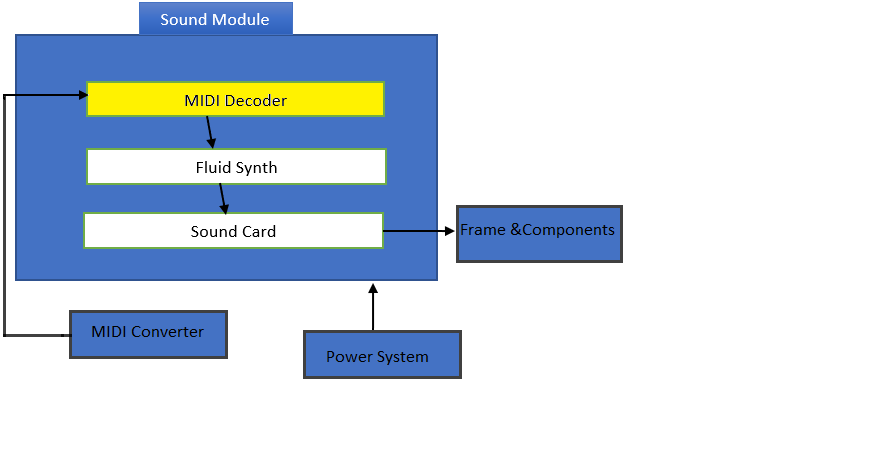
\includegraphics[width=0.60\textwidth]{images/MIDI_decoder}
 \caption{MIDI decoder subsystem diagram}
\end{figure}

\subsubsection{Assumptions}
The drivers are compatible with the raspberry pi OS. 

\subsubsection{Responsibilities}
The drivers should successfully decode the MIDI data signals to be able to be processed by the fluidsynth software. There should be no loss of data.

\subsubsection{Subsystem Interfaces}
The MIDI decoder drivers are software drivers downloaded to the raspberry pi OS. It doesn't have any sub-system inside it


\subsection{FluidSynth}
FluidSynth is a real-time software synthesizer based on the SoundFont 2 specifications and has reached widespread distribution. It converts the MIDI signals to produce desired sound waves.

\begin{figure}[h!]
	\centering
 	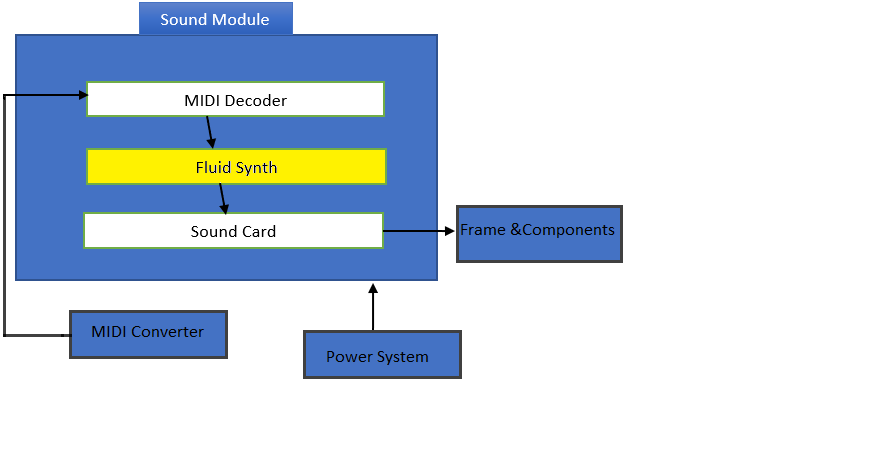
\includegraphics[width=0.60\textwidth]{images/fluidsynthpng}
 \caption{FluidSynth subsystem diagram}
\end{figure}

\subsubsection{Assumptions}
The software already has default preset sounds built-in. It also has the functionality manipulate the sound to produce various sound effects. Also it is free, open source and easy to use.

\subsubsection{Responsibilities}
The software is used to convert MIDI signals to sound waves. It should have multiple different sound effects and create a wide range of sound octaves in different formats.

\subsubsection{Subsystem Interfaces}
The software is downloaded and installed into the raspberry pi. It is supported by the raspberry pi OS.


\subsection{Sound Card}
The sound card is integrated into the raspberry pi as drivers. It converts the data outputted by FluidSynth to sound data which is released through the speaker as the final output.

\begin{figure}[h!]
	\centering
 	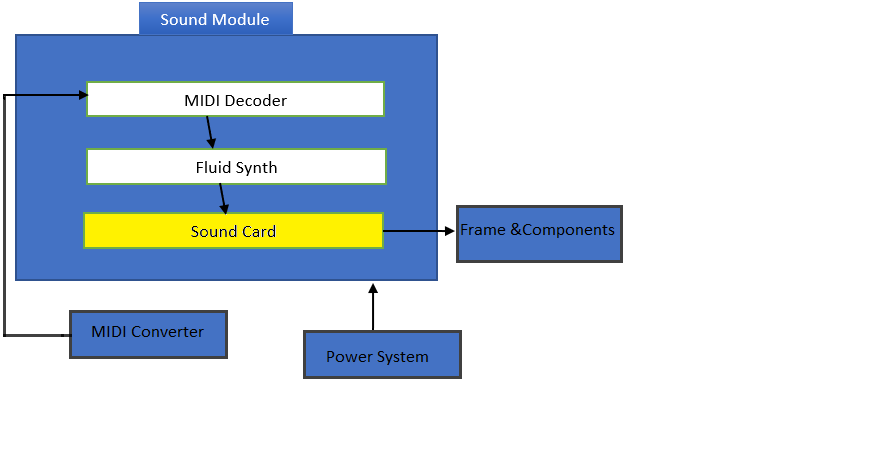
\includegraphics[width=0.60\textwidth]{images/soundcard}
 \caption{Sound Card subsystem diagram}
\end{figure}

\subsubsection{Assumptions}
The sound card drivers are already built-in and integrated to the raspberry pi.

\subsubsection{Responsibilities}
The sound card should handle decent amount of data set. It should be able to produce a wide variety of sound data with different wavelengths.

\subsubsection{Subsystem Interfaces}
The sound card drivers are built-in software built-in to the raspberry pi OS. It doesn't have any sub-system inside it.




